\documentclass{article}

\usepackage{imfellEnglish}
\usepackage[T1]{fontenc}
\usepackage{graphicx}
\usepackage{tikz}


\usepackage[landscape,margin=1cm]{geometry}

\begin{document}\pagenumbering{gobble}
\Huge
5 of me pirates want just onions.

The rest want just olives.
\begin{center}
  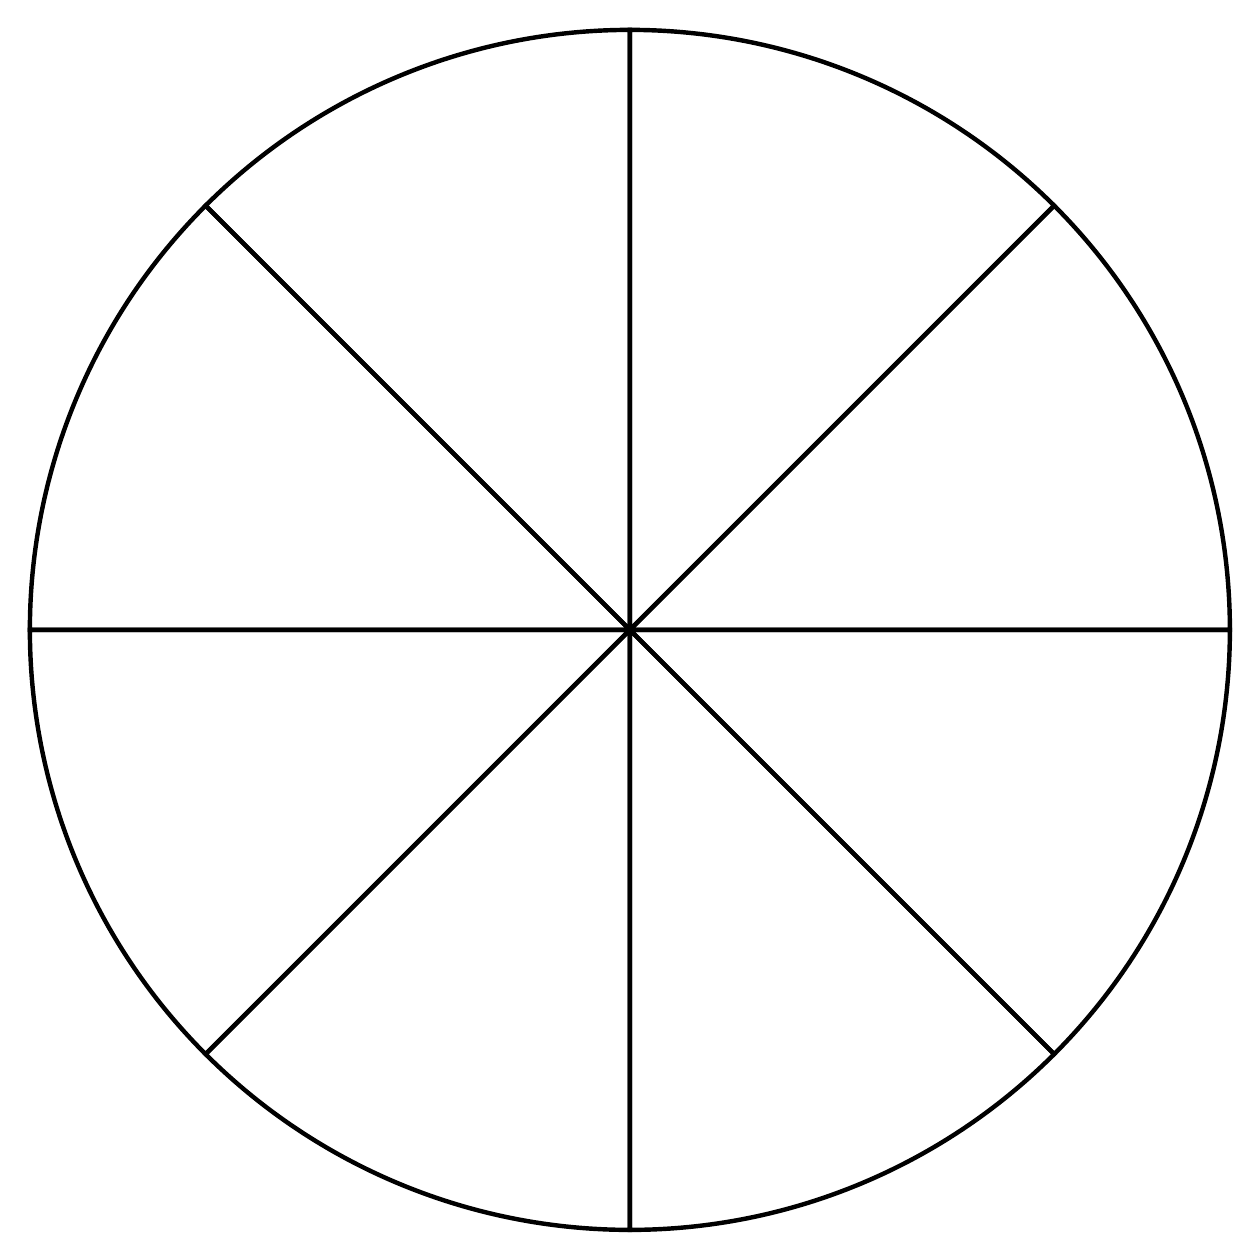
\begin{tikzpicture}[scale=2]
    \foreach \i in {1,...,8} {
    \draw[ultra thick] (0,0) -- ({45*(\i - 1)}:1.5in) arc ({45*(\i - 1)}:{45*\i}:1.5in) -- cycle;
  }
\end{tikzpicture}
\end{center}

\newpage

1 out of 4 of my pirates want just tomatoes.

  3 out of 4 want just garlic.
\begin{center}
  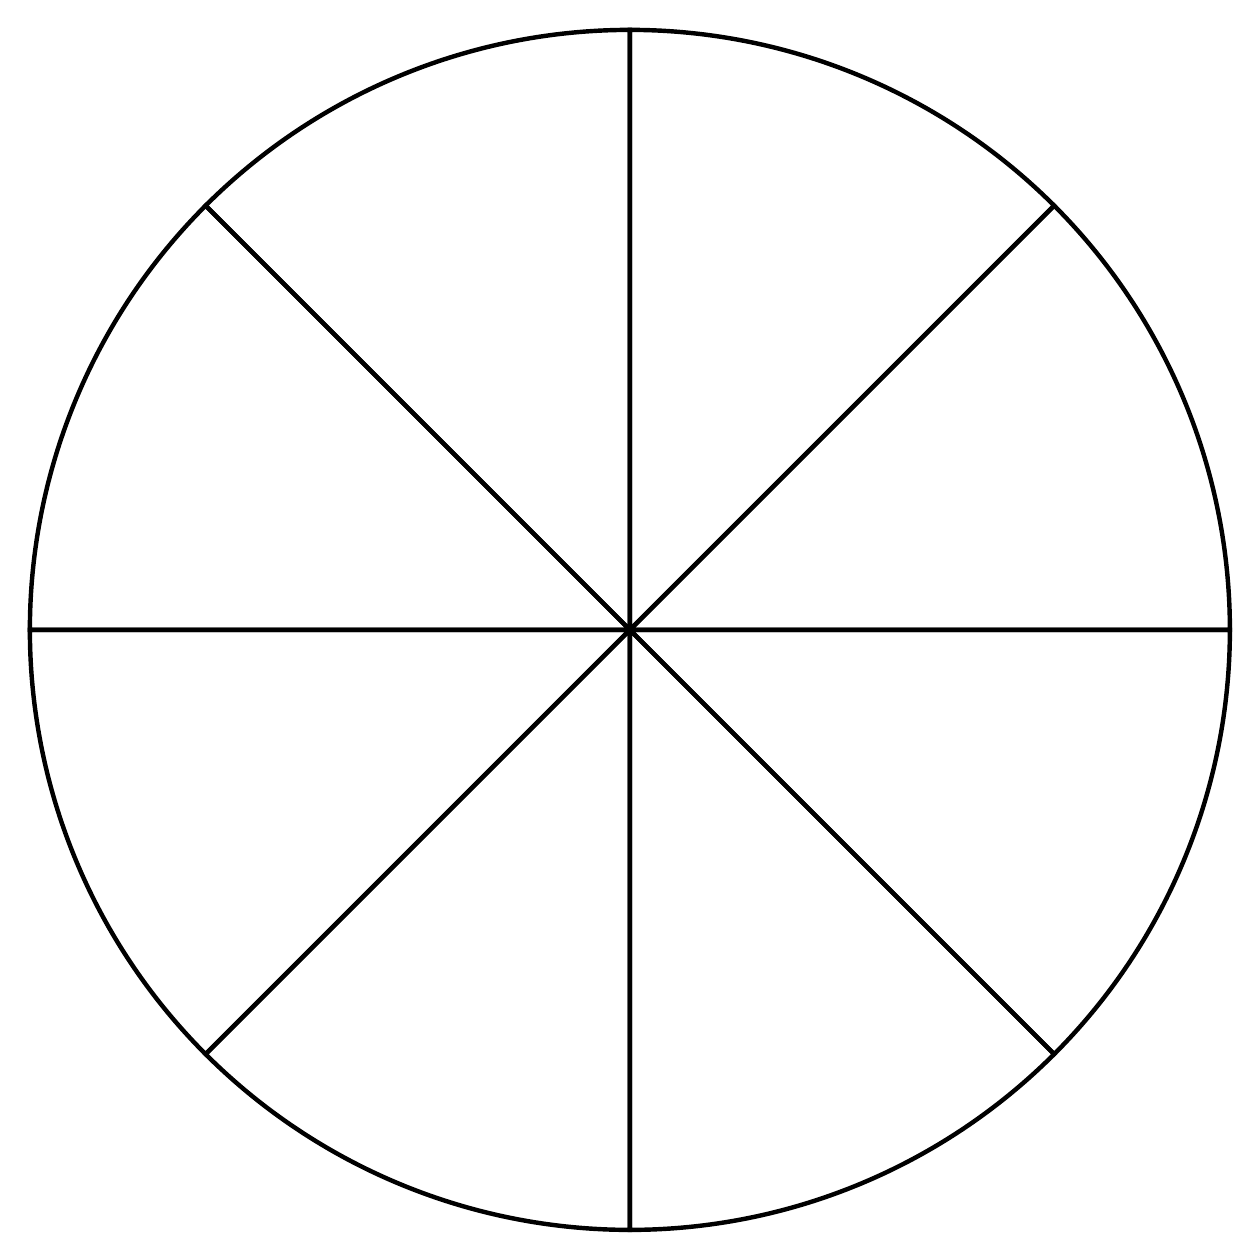
\begin{tikzpicture}[scale=2]
    \foreach \i in {1,...,8} {
    \draw[ultra thick] (0,0) -- ({45*(\i - 1)}:1.5in) arc ({45*(\i - 1)}:{45*\i}:1.5in) -- cycle;
  }
\end{tikzpicture}
\end{center}

\newpage
  1 out of 2 of my pirates want just mushrooms.

  1 out of 8 want just beets.

  3 out of 8 want just sausage.
\begin{center}
    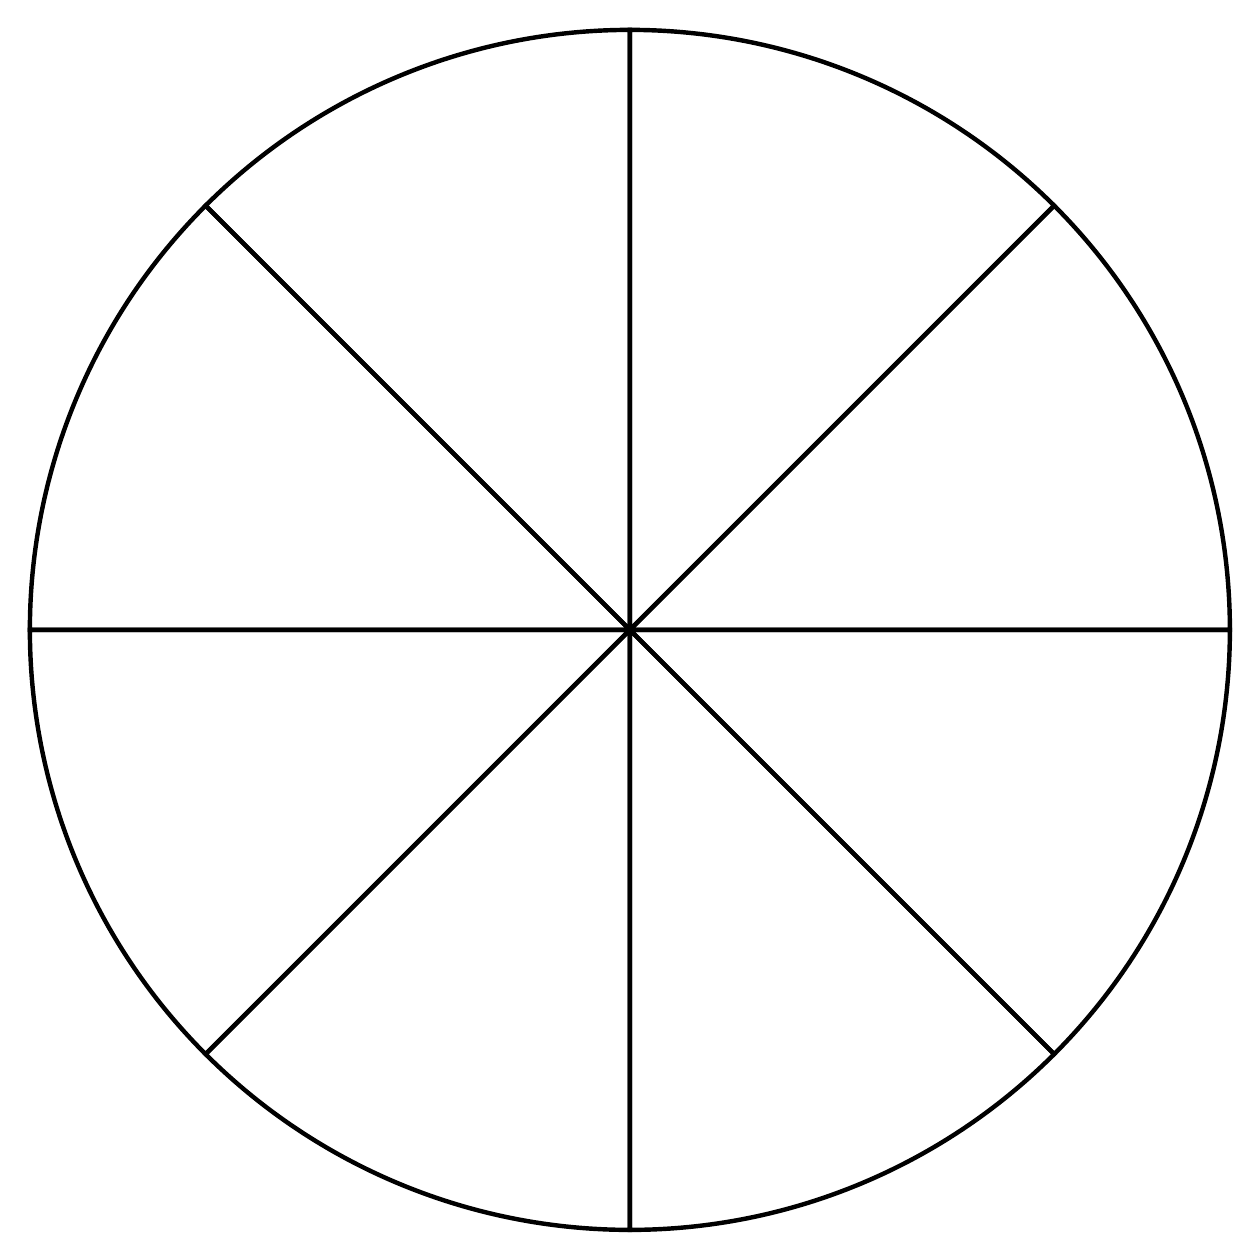
\begin{tikzpicture}[scale=2]
    \foreach \i in {1,...,8} {
    \draw[ultra thick] (0,0) -- ({45*(\i - 1)}:1.5in) arc ({45*(\i - 1)}:{45*\i}:1.5in) -- cycle;
  }
\end{tikzpicture}
\end{center}
\end{document}
